\section{Railway network}
The flatland environment is simulated by a rectangular grid of fixed size, which can be set by the user. Each cell of the grid is either a rail cell, or an empty unusable cell, or a \textbf{target} cell. Rails are of different type, depending on the available \textbf{transitions}: there are 16 different transitions in flatland, since there are 4 different orientations, and 4 other directions of exit from the cell. Thus, each cell is described by a bitmap that represents the whole transition space.\\
However, not every transition is allowed in flatland.\ Since the aim is to actually simulate a real railway system, only a maximum of 2 exit directions are allowed from every orientation of the agent, which result in 8 different cell types (including empty ones).\\ \\
Flatland offers also a \textit{sparse\_rail\_generator} that randomizes the creation of a realistic railway structure, where clusters of cities are sparsely connected to each other, allowing to mimic as faithfully as possible real city railway networks.

\begin{figure}[H] 
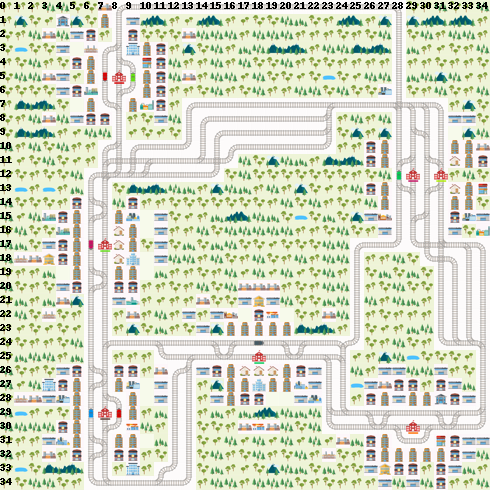
\includegraphics[height=80mm, width=80mm, scale=0.5]{chapters/sparse_railway.png}
\centering
\caption{Sparse railway}
\label{fig:s1}
\end{figure}

\section{Agents}
Trains have a number of important properties:
\begin{itemize}
\item \textbf{Position}: the current coordinates of the agent.
\item \textbf{Target}: the position of the target cell.
\item \textbf{Direction}: the current orientation described with an integer\\
    \verb|[0=North, 1=Est, 2=South, 3=West]| 
\item \textbf{Movement}: an integer describing the status of the agent\\
    \verb|[0=READY_TO_DEPART, 1=ACTIVE, 2=DONE, 3=DONE_REMOVED]|
\end{itemize}
\noindent
Since every agent is liable to malfunctions, much like real trains, there are properties to keep track of that in addition to variables that store the agents' speed:
\begin{itemize}
\item 	\textbf{Malfunction rate}: the Poisson rate at which malfunctions occur
\item \textbf{Malfunction}: a counter of the remaining time the agent will remain malfunctioning
\item \textbf{Next malfunction}: number of steps until next malfunction
\item \textbf{Number of malfunctions}: the total number of malfunctions for this agent
\item \textbf{Max speed}: a fraction between 0 and 1. (\textit{e.g.} a speed of 1/2 means that the agent changes cell after 2 time steps)
\item \textbf{Position fraction}: related to speed, indicates when the next action can be taken
\end{itemize}

\section{Our environment}